\documentclass[11pt,a4paper]{article}
\usepackage[margin=19mm]{geometry}
\usepackage[T1]{fontenc}
\usepackage{mathptmx}
\usepackage{graphicx}
\usepackage{booktabs}
\usepackage{hyperref}
\usepackage{microtype}
\usepackage{parskip}
\hypersetup{pdftitle={MIMESIS: Project brief},pdfauthor={Arjun Vijay Prakash},colorlinks=true,urlcolor=black}
\setlength{\parskip}{6pt}
\begin{document}
{\LARGE\bfseries MIMESIS}\par
{\large Which Earth landscape does the terrain comparison actually select?}\par
Arjun Vijay Prakash, Grade XI\quad City Montessori School, Kanpur Road, Lucknow, India

\textbf{Challenge.} Identify Earth locations that can help prepare for permanent Moon bases and Mars exploration. MIMESIS focuses on regional terrain mapping and the reliability of the location choice.

\textbf{What we built.} A four-view explorer connects NASADEM Earth terrain with MOLA Mars and LOLA Moon measurements. Source-linked exports, a reproducible analysis and a ten-page paper accompany the application. The geographic study compares 3,693 overlapping Namib and Atacama windows against six targets under two scoring contracts and two analysis supports.

\begin{center}
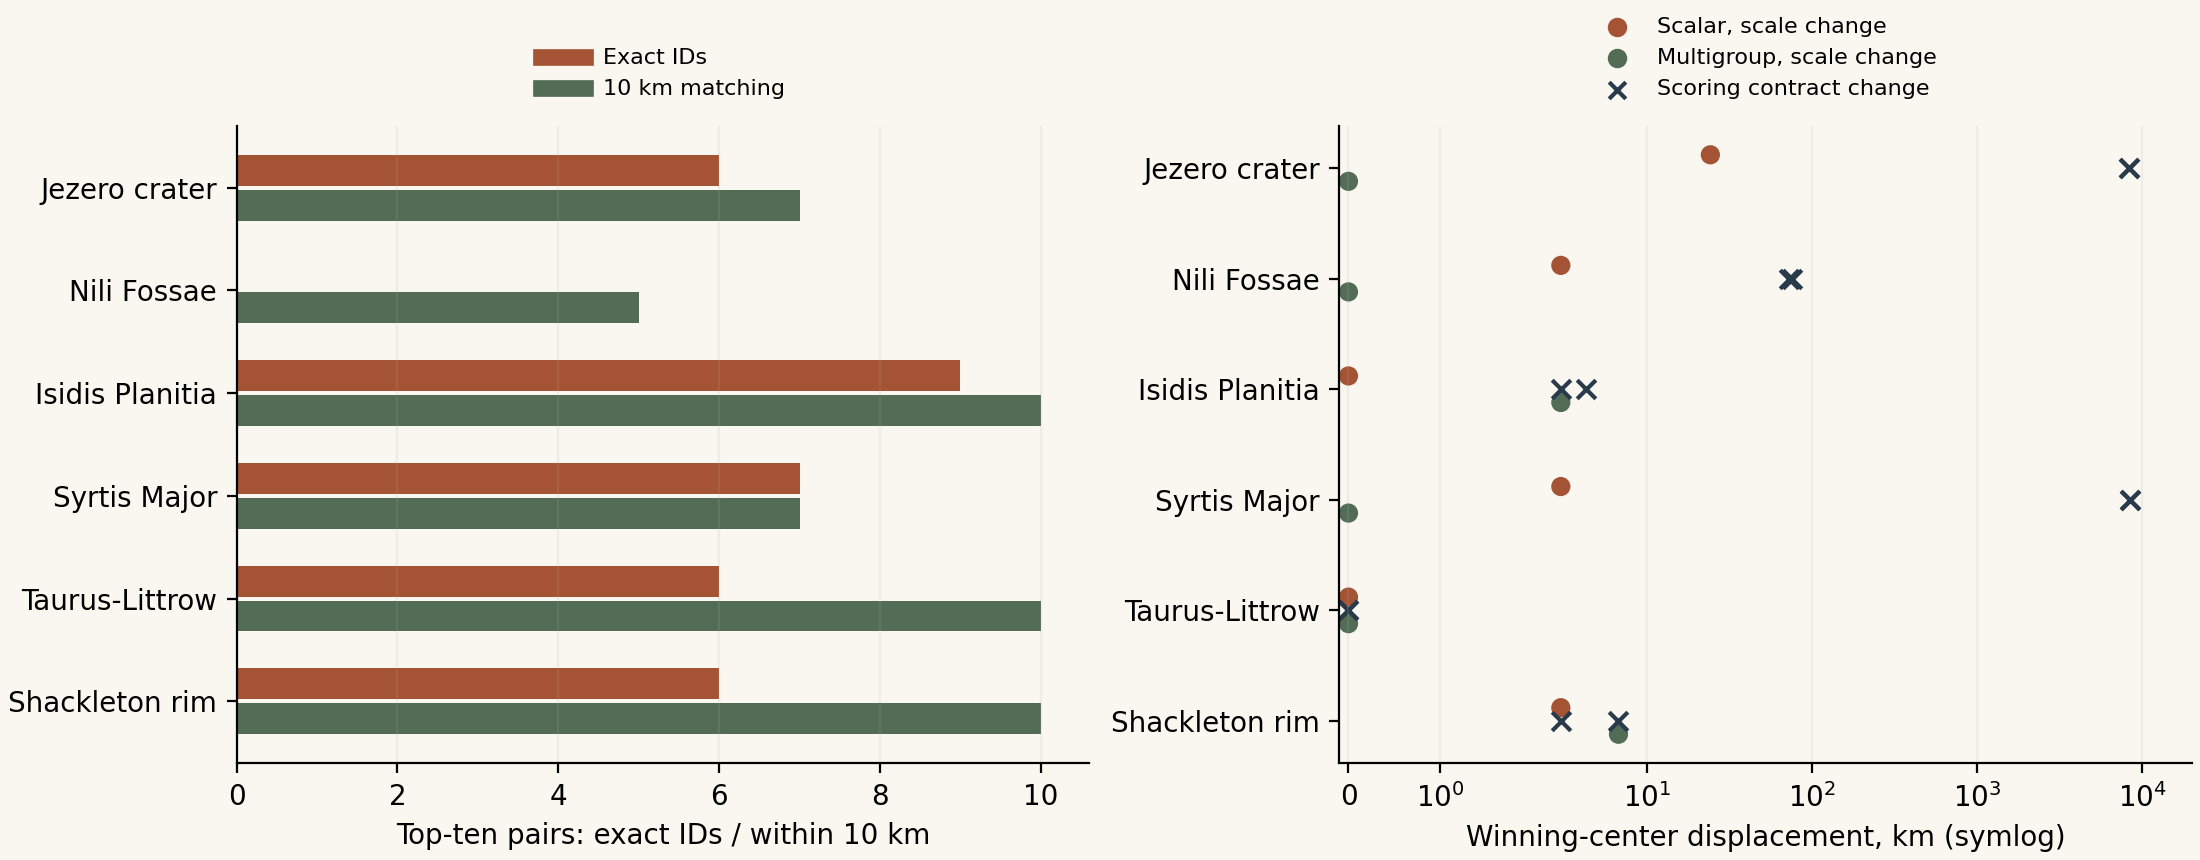
\includegraphics[width=\linewidth]{../paper/site-stability.png}
\end{center}

\textbf{Finding 1: changed ranks can share ground.} Nili Fossae has zero identical top-ten windows across supports, yet its winning centers are only 3 km apart and their footprint intersection-over-union is 73.9\%. Five top-ten pairs can be matched one-to-one within 10 km.

\textbf{Finding 2: scoring assumptions can change the continent.} Support changes move winning centers by at most 24.2 km. Changing the scoring contract moves Jezero and Syrtis winners between Namibia and Chile, by 8,349--8,484 km. This compares whole contracts; it does not isolate one causal feature or prove that either method is better.

\textbf{What this enables.} Users can distinguish numerical turnover from geographic replacement, inspect assumption-dependent choices and export terrain candidates for a follow-up desk study. The intended benefit is better-targeted investigation; mission savings and improved task performance have not been measured.

\vfill
\href{https://github.com/ArjunCodess/MIMESIS}{github.com/ArjunCodess/MIMESIS}\hfill Lucknow local event, NASA Space Apps 2026
\newpage
{\Large\bfseries Evidence for the judging criteria}

\textbf{Impact.} A mapping team can inspect candidate footprints and source records before investing in detailed investigation. Geographic exports work with ordinary GIS tools. Field access, safety and utility remain to be established.

\textbf{Creativity.} MIMESIS connects ranking sensitivity to physical geography: zero shared identifiers need not mean entirely different ground, while an apparently stable ranking can depend strongly on the scoring contract. These are new measured project results, with no claim that sensitivity analysis or geographic matching was invented here.

\textbf{Validity.} Both scoring contracts, all targets and every matching radius are retained. Maximum-cardinality one-to-one matching prevents duplicate counting. Source and implementation hashes make the calculation inspectable. Nine focused scientific and API tests check physical behavior, evidence boundaries and integration. Software checks do not validate geology.

\textbf{Relevance.} NASADEM, MOLA and LOLA supply the actual descriptors used to compare Earth, Mars and the Moon. Related LROC pit and MOLA point-support experiments expose source limitations. The output is a target-specific Earth-location shortlist for regional terrain mapping, not a general habitability or base-safety score.

\textbf{Presentation.} Start with a planetary target in Explore. In Evidence, show Nili's rank turnover and geographic continuity, then Jezero's contract-dependent continent change. Download the GeoJSON and open the paper. The project includes the full 90-second demonstration script in \texttt{submission.md}.

\textbf{A location example.} The scalar cross-support shortlist for Nili Fossae is centered at $25.16248^\circ$ S, $16.05951^\circ$ E in Namibia, with ranks 17 and 19. That weak compromise is reported rather than hidden. The location is a 20 km analysis window, not a verified geological feature or approved field site. Both lunar targets also have exported Chilean terrain candidates, whose atmosphere, gravity and polar illumination differ from the Moon.

\textbf{Novelty boundary and next scientific step.} The project establishes a descriptive geographic result in two previously inspected regional pools. It does not establish a previously unrecognized geological analogue, independent rehearsal benefit or world-first method. A stronger geological claim needs registered process-relevant positive and negative reference areas, source-quality evidence and independent outcomes for a declared mapping task. The separate cave pilot still requires verified rims and source qualification.

\textbf{Reproduce.} Install the project as described in the repository README, then run \path{python scripts/measure_site_stability.py}. No new download is needed for this descriptor-level analysis. Raw DEM reconstruction and geological validation are separate tasks.

\textbf{Authorship and sources.} Arjun Vijay Prakash built MIMESIS; Codex assisted with implementation, analysis code and writing. The research paper and source manifests retain observation provenance, baseline-method citations and original license terms. No NASA endorsement, peer review or independent expert assessment is claimed.

\vfill
\href{https://github.com/ArjunCodess/MIMESIS}{github.com/ArjunCodess/MIMESIS}\hfill \href{https://arjuncodess.is-a.dev/}{arjuncodess.is-a.dev}
\end{document}
